\documentclass[a4paper, 11pt, oneside]{article}

\usepackage[utf8]{inputenc}
\usepackage[T1]{fontenc}
\usepackage[french]{babel}
\usepackage{array}
\usepackage{shortvrb}
\usepackage{listings}
\usepackage[fleqn]{amsmath}
\usepackage{amsfonts}
\usepackage{fullpage}
\usepackage{enumerate}
\usepackage{graphicx}             % import, scale, and rotate graphics
\usepackage{subfigure}            % group figures
\usepackage{alltt}
\usepackage{url}
\usepackage{indentfirst}
\usepackage{eurosym}
\usepackage{listings}
\usepackage{color}
\usepackage[table,xcdraw,dvipsnames]{xcolor}

% Change le nom par défaut des listing
\renewcommand{\lstlistingname}{Extrait de Code}

% Change la police des titres pour convenir à votre seul lecteur
\usepackage{sectsty}
\allsectionsfont{\sffamily\mdseries\upshape} 
% Idem pour la table des matière.
\usepackage[nottoc,notlof,notlot]{tocbibind} 
\usepackage[titles,subfigure]{tocloft} 
\renewcommand{\cftsecfont}{\rmfamily\mdseries\upshape}
\renewcommand{\cftsecpagefont}{\rmfamily\mdseries\upshape} 

\definecolor{mygray}{rgb}{0.5,0.5,0.5}
\newcommand{\coms}[1]{\textcolor{MidnightBlue}{#1}}

\lstset{
    language=C, % Utilisation du langage C
    commentstyle={\color{MidnightBlue}}, % Couleur des commentaires
    frame=single, % Entoure le code d'un joli cadre
    rulecolor=\color{black}, % Couleur de la ligne qui forme le cadre
    stringstyle=\color{RawSienna}, % Couleur des chaines de caractères
    numbers=left, % Ajoute une numérotation des lignes à gauche
    numbersep=5pt, % Distance entre les numérots de lignes et le code
    numberstyle=\tiny\color{mygray}, % Couleur des numéros de lignes
    basicstyle=\tt\footnotesize, 
    tabsize=3, % Largeur des tabulations par défaut
    keywordstyle=\tt\bf\footnotesize\color{Sepia}, % Style des mots-clés
    extendedchars=true, 
    captionpos=b, % sets the caption-position to bottom
    texcl=true, % Commentaires sur une ligne interprétés en Latex
    showstringspaces=false, % Ne montre pas les espace dans les chaines de caractères
    escapeinside={(>}{<)}, % Permet de mettre du latex entre des <( et )>.
    inputencoding=utf8,
    literate=
  {á}{{\'a}}1 {é}{{\'e}}1 {í}{{\'i}}1 {ó}{{\'o}}1 {ú}{{\'u}}1
  {Á}{{\'A}}1 {É}{{\'E}}1 {Í}{{\'I}}1 {Ó}{{\'O}}1 {Ú}{{\'U}}1
  {à}{{\`a}}1 {è}{{\`e}}1 {ì}{{\`i}}1 {ò}{{\`o}}1 {ù}{{\`u}}1
  {À}{{\`A}}1 {È}{{\`E}}1 {Ì}{{\`I}}1 {Ò}{{\`O}}1 {Ù}{{\`U}}1
  {ä}{{\"a}}1 {ë}{{\"e}}1 {ï}{{\"i}}1 {ö}{{\"o}}1 {ü}{{\"u}}1
  {Ä}{{\"A}}1 {Ë}{{\"E}}1 {Ï}{{\"I}}1 {Ö}{{\"O}}1 {Ü}{{\"U}}1
  {â}{{\^a}}1 {ê}{{\^e}}1 {î}{{\^i}}1 {ô}{{\^o}}1 {û}{{\^u}}1
  {Â}{{\^A}}1 {Ê}{{\^E}}1 {Î}{{\^I}}1 {Ô}{{\^O}}1 {Û}{{\^U}}1
  {œ}{{\oe}}1 {Œ}{{\OE}}1 {æ}{{\ae}}1 {Æ}{{\AE}}1 {ß}{{\ss}}1
  {ű}{{\H{u}}}1 {Ű}{{\H{U}}}1 {ő}{{\H{o}}}1 {Ő}{{\H{O}}}1
  {ç}{{\c c}}1 {Ç}{{\c C}}1 {ø}{{\o}}1 {å}{{\r a}}1 {Å}{{\r A}}1
  {€}{{\euro}}1 {£}{{\pounds}}1 {«}{{\guillemotleft}}1
  {»}{{\guillemotright}}1 {ñ}{{\~n}}1 {Ñ}{{\~N}}1 {¿}{{?`}}1
}
\newcommand{\tablemat}{~}

%%%%%%%%%%%%%%%%% TITRE %%%%%%%%%%%%%%%%
\newcommand{\intitule}{Projet 2}
\newcommand{\GrNbr}{10}
\newcommand{\PrenomUN}{Cyril}
\newcommand{\NomUN}{RUSSE}
\renewcommand{\tablemat}{\tableofcontents}

%%%%%%%% ZONE PROTÉGÉE : MODIFIEZ UNE DES DIX PROCHAINES %%%%%%%%
%%%%%%%%            LIGNES POUR PERDRE 2 PTS.            %%%%%%%%
\title{INFO0947: \intitule\\ Types Abstraits de Données}
\author{Groupe \GrNbr : \PrenomUN~\textsc{\NomUN}}
\date{}
\begin{document}
\maketitle
\newpage
\tablemat
\newpage
%%%%%%%%%%%%%%%%%%%% FIN DE LA ZONE PROTÉGÉE %%%%%%%%%%%%%%%%%%%%

%%%%%%%%%%%%%%%% RAPPORT %%%%%%%%%%%%%%%

\section{\textbf{Introduction}}

\subsection{\textbf{Contexte}}

En référence à la BD Astérix et Obelix, "Le tour de Gaule d'Astérix", ce travail a pour 
but d'implémenter ce fameux tour sous la forme d'un type abstrait de données.

\subsection{\textbf{Enoncé}}
\subsubsection{Types abstraits}
Dans le cadre de ce projet, nous avions pour consigne de spécifier deux types abstraits : 
\begin{enumerate}
    \item \textbf{Ville} \\
    Ce type abstrait doit permettre de :
    \begin{itemize}
        \item créer une ville à partir de ses deux coordonnées X et Y et de son nom ;
        \item obtenir la coordonnée X d’une escale ;
        \item obtenir la coordonnée Y d’une escale ;
        \item obtenir le nom de la ville ;
        \item calculer la distance géographique entre deux ville ;
        \item enregistrer la spécialité gastronomique de la ville ;
        \item obtenir la spécialité gastronomique de la ville ;
    \end{itemize}
    \item \textbf{Gaule}\\
    Ce type abstrait doit permettre de :
    \begin{itemize}
        \item créer un tour de Gaule sur base de deux villes. Par définition, un tour 
        nouvellement créé ne peut pas constituer un circuit ;
        \item déterminer si un tour de Gaule constitue un circuit ;
        \item déterminer le nombre de villes visitées durant le tour ;
        \item déterminer le nombre totale de spécialités gastronimiques dans le tour ;
        \item déterminer la spécialité gastronomique d’une ville du tour ;
        \item ajouter une ville à un tour ;
        \item supprimer une ville d’un tour ;
    \end{itemize}
\end{enumerate}

\subsubsection{Représentation Concrète}

Ces types abstraits doivent être représentés de 2 manières :
\begin{itemize}
    \item Un tableau
    \item Une liste chainée
\end{itemize}

\section{\textbf{Signature des TAD}}

\subsection{\textbf{Ville}}

\noindent Type :
\begin{itemize}
    \item Ville
\end{itemize}
\noindent Utilise :
\begin{itemize}
    \item $String$
    \item $\mathbb{R}$
\end{itemize}
\noindent Opérations :
\begin{itemize}
    \item creer\_ville : $String \times \mathbb{R} \times \mathbb{R} \rightarrow Ville$
    \item get\_x\_ville : $Ville \rightarrow \mathbb{R}$
    \item get\_y\_ville : $Ville \rightarrow \mathbb{R}$
    \item get\_nom\_ville : $Ville \rightarrow String$
    \item get\_specialite\_ville : $Ville \rightarrow String$
    \item set\_specialite\_ville : $Ville \times String \rightarrow Ville$
    \item distance\_entre\_2\_villes : $Ville \times Ville \rightarrow \mathbb{R}$
\end{itemize}
\noindent Préconditions :
\begin{itemize}
    \item $\emptyset$
\end{itemize}
\noindent Axiomes : $\forall x,y \in \mathbb{R} \wedge \forall V_1, V_2 \in Ville \wedge \forall s,t \in String$
\begin{itemize}
    \item distance\_entre\_2\_villes($V_1,V_2$) = 
    \\$\sqrt{(get\_x\_ville(V_2)-get\_x\_ville(V_1))^2+(get\_y\_ville(V_2)-get\_y\_ville(V_1))^2}$
    \item distance\_entre\_2\_villes(set\_specialite\_ville($V_1, s$), set\_specialite\_ville($V_2, t$)) = \\
    distance\_entre\_2\_villes($V_1,V_2$)
    \item get\_x\_ville(creer\_ville($s, x, y$)) = $x$
    \item get\_y\_ville(creer\_ville($s, x, y$)) = $y$
    \item get\_x\_ville(set\_specialite\_ville($V_1, s$)) = get\_x\_ville($V_1$)
    \item get\_y\_ville(set\_specialite\_ville($V_1, s$)) = get\_y\_ville($V_1$)
    \item get\_nom\_ville(creer\_ville($s, x, y$)) = $s$
    \item get\_nom\_ville(set\_specialite\_ville($V_1, s$)) = get\_nom\_ville($V_1$)
    \item get\_specialite\_ville(set\_specialite\_ville($V_1, s$)) = $s$
    \item get\_specialite\_ville(creer\_ville($s, x, y$)) = NULL

\end{itemize}

\subsection{\textbf{Gaule}}
\noindent Type :
\begin{itemize}
    \item Gaule
\end{itemize}

\noindent Utilise :
\begin{itemize}
    \item $Ville$
    \item $Entiers$
    \item $String$
    \item $Booleen$
\end{itemize}

\noindent Opérations :
\begin{itemize}
    \item cree\_nouveau\_tour : $Ville \times Ville \rightarrow Gaule$
    \item get\_nombre\_villes : $Gaule \rightarrow Entiers$
    \item ajoute\_ville : $Gaule \times Ville \rightarrow Gaule$
    \item supprime\_ville : $Gaule \rightarrow Gaule$
    \item get\_est\_circuit : $Gaule \rightarrow Booleen$
    \item get\_nombre\_specialite : $Gaule \rightarrow Entiers$
    \item get\_specialite : $Gaule \times String \rightarrow String$
    \item ville\_en\_double : $Gaule \times Ville \rightarrow Booleen$
\end{itemize}

\noindent Préconditions :

\noindent Axiomes :$\forall G \in Gaule, \forall V_1, V_2, \in Ville$
\begin{itemize}
    \item get\_nombre\_villes(ajoute\_ville($G, V_1$)) = get\_nombre\_villes($G$)+1
    \item get\_nombre\_villes(supprime\_ville($G$)) = get\_nombre\_villes($G$)-1 
    \\si get\_nombre\_villes($G$)$>0$ 
    \\sinon get\_nombre\_villes(supprime\_ville($G$)) = get\_nombre\_villes($G$)
    \item get\_nombre\_villes(cree\_nouveau\_tour($V_1, V_2$)) = 2
    \item get\_nombre\_specialite(ajoute\_ville($G, V_1$)) = get\_nombre\_specialite($G$)+1
    \\si ville\_en\_double($G, V_1$)=False $\wedge$ get\_specialite($G, V_1$)$\ne$NULL
    \\sinon get\_nombre\_specialite(ajoute\_ville($G, V_1$)) = get\_nombre\_specialite($G$)
    \item get\_nombre\_specialite(cree\_nouveau\_tour($V_1, V_2$)) = 2
    \\si get\_specialite($G, V_1$)$\ne$NULL $\wedge$ get\_specialite($G, V_2$)$\ne$NULL
    \item get\_nombre\_specialite(cree\_nouveau\_tour($V_1, V_2$)) = 1
    \\si get\_specialite($G, V_1$)$\ne$NULL $\wedge$ get\_specialite($G, V_2$)=NULL
    \\$\vee$get\_specialite($G, V_2$)$\ne$NULL $\wedge$ get\_specialite($G, V_1$)=NULL
    \item get\_nombre\_specialite(cree\_nouveau\_tour($V_1, V_2$)) = 0
    \\si get\_specialite($G, V_1$)=NULL $\wedge$ get\_specialite($G, V_2$)=NULL
    \item get\_est\_circuit(cree\_nouveau\_tour($V_1, V_2$)) = False
    \item get\_specialite(cree\_nouveau\_tour($V_1, V_2$), $V_1$) =  get\_specialite\_ville($V_1$)
    \item get\_specialite(cree\_nouveau\_tour($V_1, V_2$), $V_2$) =  get\_specialite\_ville($V_2$)
    \item get\_specialite(ajoute\_ville($G, V_1$), $V_1$) = get\_specialite\_ville($V_1$)
\end{itemize}

\section{\textbf{Spécifications des TAD}}

\subsection{\textbf{Ville}}
\subsubsection{Structure}
\begin{lstlisting}[caption = {Structure "Ville"}]
    struct Ville_t{
    char *nom;
    float x;
    float y;
    char *specialite;
    };
\end{lstlisting}

\subsubsection{Spécification des fonctions et procédures de ville.h}
\begin{lstlisting}[caption = {Spécification des fonctions et procédures du header "ville.h"}]
    /*
    *@pre : (>\color{MidnightBlue}$nom \ne NULL \wedge x=x_0\wedge y=y_0 \wedge nom=nom_0$<)
    *@post : (>\color{MidnightBlue}$ville_{init}\wedge  x=x_0\wedge y=y_0 \wedge nom=nom_0\wedge get\_x\_ville(ville)=ville->x\wedge$<)
    *(>\color{MidnightBlue}$get\_y\_ville(ville)=ville->y \wedge get\_nom\_ville(ville)=ville->nom$<)
    */
    Ville *creer_ville(char *nom, float x, float y);

    /*
    *@pre : (>\color{MidnightBlue}$\emptyset$<)
    *@post : (>\color{MidnightBlue}$ville=NULL$<)
    */
    void detruit_ville(Ville *ville);
    
    /*
    *@pre : (>\color{MidnightBlue}$ville\ne NULL$<)
    *@post : (>\color{MidnightBlue}$ville=ville_0 \wedge get\_x\_ville(ville)=ville->x$<)
    */
    float get_x_ville(Ville *ville);
    
    /*
    *@pre : (>\color{MidnightBlue}$ville\ne NULL$<)
    *@post : (>\color{MidnightBlue}$ville=ville_0 \wedge get\_y\_ville(ville)=ville->y$<)
    */
    float get_y_ville(Ville *ville);
    
    /*
    *@pre : (>\color{MidnightBlue}$ville\ne NULL$<)
    *@post : (>\color{MidnightBlue}$ville=ville_0 \wedge get\_nom\_ville(ville)=ville->nom$<)
    */
    char *get_nom_ville(Ville *ville);
    
    /*
    *@pre : (>\color{MidnightBlue}$ville\ne NULL$<)
    *@post : (>\color{MidnightBlue}$ville=ville_0 \wedge get\_specialite\_ville(ville)=ville->specialite$<)
    */
    char *get_specialite_ville(Ville *ville);
    
    /*
    *@pre : (>\color{MidnightBlue}$ville\ne NULL \wedge specialite\ne NULL\wedge specialite = specialite_0$<)
    *@post : (>\color{MidnightBlue}$ville=ville_0\wedge specialite = specialite_0 \wedge get\_specialite\_ville(ville)=specialite$<)
    */
    void set_specialite_ville(Ville *ville, char *specialite);
    
    /*
    *@pre : (>\color{MidnightBlue}$ville1=ville1_0\ne NULL \wedge ville2=ville2_0\ne NULL $<)
    *@post : (>\color{MidnightBlue}$ville1=ville1_0 \wedge ville2=ville2_0\wedge $<)
    *(>\color{MidnightBlue}$distance\_entre\_2\_villes(ville1,ville2) = $<)
    *(>\color{MidnightBlue}$\sqrt{(get\_x\_ville(ville2)-get\_x\_ville(ville1))^2+(get\_y\_ville(ville2)-get\_y\_ville(ville1))^2}$<)
    */
    float distance_entre_2_villes(Ville *ville1, Ville *ville2);
    
    /*
    *@pre : (>\color{MidnightBlue}$\emptyset$<)
    *@post : (>\color{MidnightBlue}retourne la taille mémoire de la struct Ville<)
    */
    int size_ville(void);
\end{lstlisting}

\subsection{\textbf{Gaule}}
\subsubsection{Structure en Tableau}
\begin{lstlisting}[caption = {Structure "Gaule" dans l'implémentation en tableau}]
    struct Gaule_t{
    Ville **tableau_ville;
    int nombre_villes;
    int est_circuit;
    int nombre_specialites;
    };
\end{lstlisting}



\subsubsection{Structure en Liste chainée}
    Pour la liste chainée, une deuxième structure vient s'ajouter. La première, comme pour les tableaux, 
    garde les informations sur la liste et la deuxième sont les structures qui correspondront chacune à une 
    des villes avec un pointeur sur l'élément suivant et précédent de la liste.
\begin{lstlisting}[caption = {Structure "Gaule" dans l'implémentation en tableau}]
    struct Gaule_t{
    Cellule_Gaule *premiere_cellule;
    Cellule_Gaule *derniere_cellule;
    int nombre_villes;
    int est_circuit;
    int nombre_specialites;
    };

    struct Cellule_Gaule_t{
    Cellule_Gaule *cellule_suivante;
    Cellule_Gaule *cellule_precedente;
    Ville *ville;
    };
\end{lstlisting}

\subsubsection{Spécification des fonctions et procédures gaule.h}

\begin{lstlisting}[caption = {Spécification des fonctions et procédures du header "gaule.h"}]
    /*
    *@pre : (>\color{MidnightBlue}$ville1=ville1_0\ne NULL \wedge ville2=ville2_0\ne NULL $<)
    *@post : (>\color{MidnightBlue}$ville1=ville1_0 \wedge ville2=ville2_0\wedge tour_{init}$<)
    */
    Gaule *cree_nouveau_tour(Ville *ville1, Ville *ville2);

    /*
    *@pre : (>\color{MidnightBlue}$\emptyset$<)
    *@post : (>\color{MidnightBlue}$tour=NULL$<)
    */
    void detruit_tour(Gaule *tour);

    /*
    *@pre : (>\color{MidnightBlue}$tour\ne NULL \wedge nombre\_villes>0$<)
    *@post : (>\color{MidnightBlue}$get\_nombre\_villes(tour)=nombre\_villes$<)
    */
    void set_nombre_villes(Gaule *tour, int nombre_villes);

    /*
    *@pre : (>\color{MidnightBlue}$tour\ne NULL$<)
    *@post : (>\color{MidnightBlue}$get\_nombre\_villes = get\_nombre\_villes(tour)$<)
    */
    int get_nombre_villes(Gaule *tour);

    /*
    *@pre : (>\color{MidnightBlue}$tour\ne NULL \wedge ville\ne NULL$<)
    *@post : (>\color{MidnightBlue}$get\_nombre\_villes(ajoute\_ville(tour, ville)) = get\_nombre\_villes(tour)+1\wedge$<)
    *ville ajoutée à tour
    */
    int ajoute_ville(Gaule *tour, Ville *ville);

    /*
    *@pre : (>\color{MidnightBlue}$tour\ne NULL \wedge get\_nombre\_villes(tour)>0$<)
    *@post : dernière ville retirée de tour 
    *(>\color{MidnightBlue}$\wedge get\_nombre\_villes(tour)=get\_nombre\_villes(tour_0)-1$<)
    */
    void supprime_ville(Gaule *tour);

    /*
    *@pre : (>\color{MidnightBlue}$\emptyset$<)
    *@post : (>\color{MidnightBlue}$compare_string(chaine1, chaine2)=0 si chaine1=chaine2, -1 sinon$<)
    */
    int compare_string(char *chaine1, char *chaine2);

    /*
    *@pre : (>\color{MidnightBlue}$tour\ne NULL$<)
    *@post : (>\color{MidnightBlue}$get\_est\_circuit(tour)=1 $<)
    *si premiere ville et derniere ville de tour sont les mêmes
    */
    void maj_est_circuit(Gaule *tour);

    /*
    *@pre : (>\color{MidnightBlue}$tour\ne NULL$<)
    *@post : retourne tour->est\_circuit
    */
    int get_est_circuit(Gaule *tour);

    /*
    *@pre : (>\color{MidnightBlue}$tour\ne NULL$<)
    *@post : retourne tour_>nombre\_specialites
    */
    int get_nombre_specialites(Gaule *tour);

    /*
    *@pre : (>\color{MidnightBlue}$tour\ne NULL \wedge nom\_ville\ne NULL$<)
    *@post : (>\color{MidnightBlue}$\exists V_1\in Ville, get\_nom\_ville(Ville)=nom\_ville\implies get\_specialite(tour, nom\_ville)=$<)
    *(>\color{MidnightBlue}$get\_specialite\_ville(V_1)$<)
    */
    char *get_specialite(Gaule *tour, char *nom_ville);

    /*
    *@pre : (>\color{MidnightBlue}$tour\ne NULL \wedge nom\_ville\ne NULL$<)
    *@post : (>\color{MidnightBlue}$ville\_en\_double(tour, nom\_ville)=1,$<)
    *(>\color{MidnightBlue}$\exists V_1,V_2 \in Ville, V_1,V_2\subset tour \wedge get\_nom\_ville(V_1)=get\_nom\_ville(V_2)$<)
    *sinon (>\color{MidnightBlue}$ville\_en\_double(tour, nom\_ville)=0$<)
    */
    int ville_en_double(Gaule *tour, char *nom_ville);
\end{lstlisting}

\subsubsection{Schématisation}
\begin{figure}[h]
    \centering
    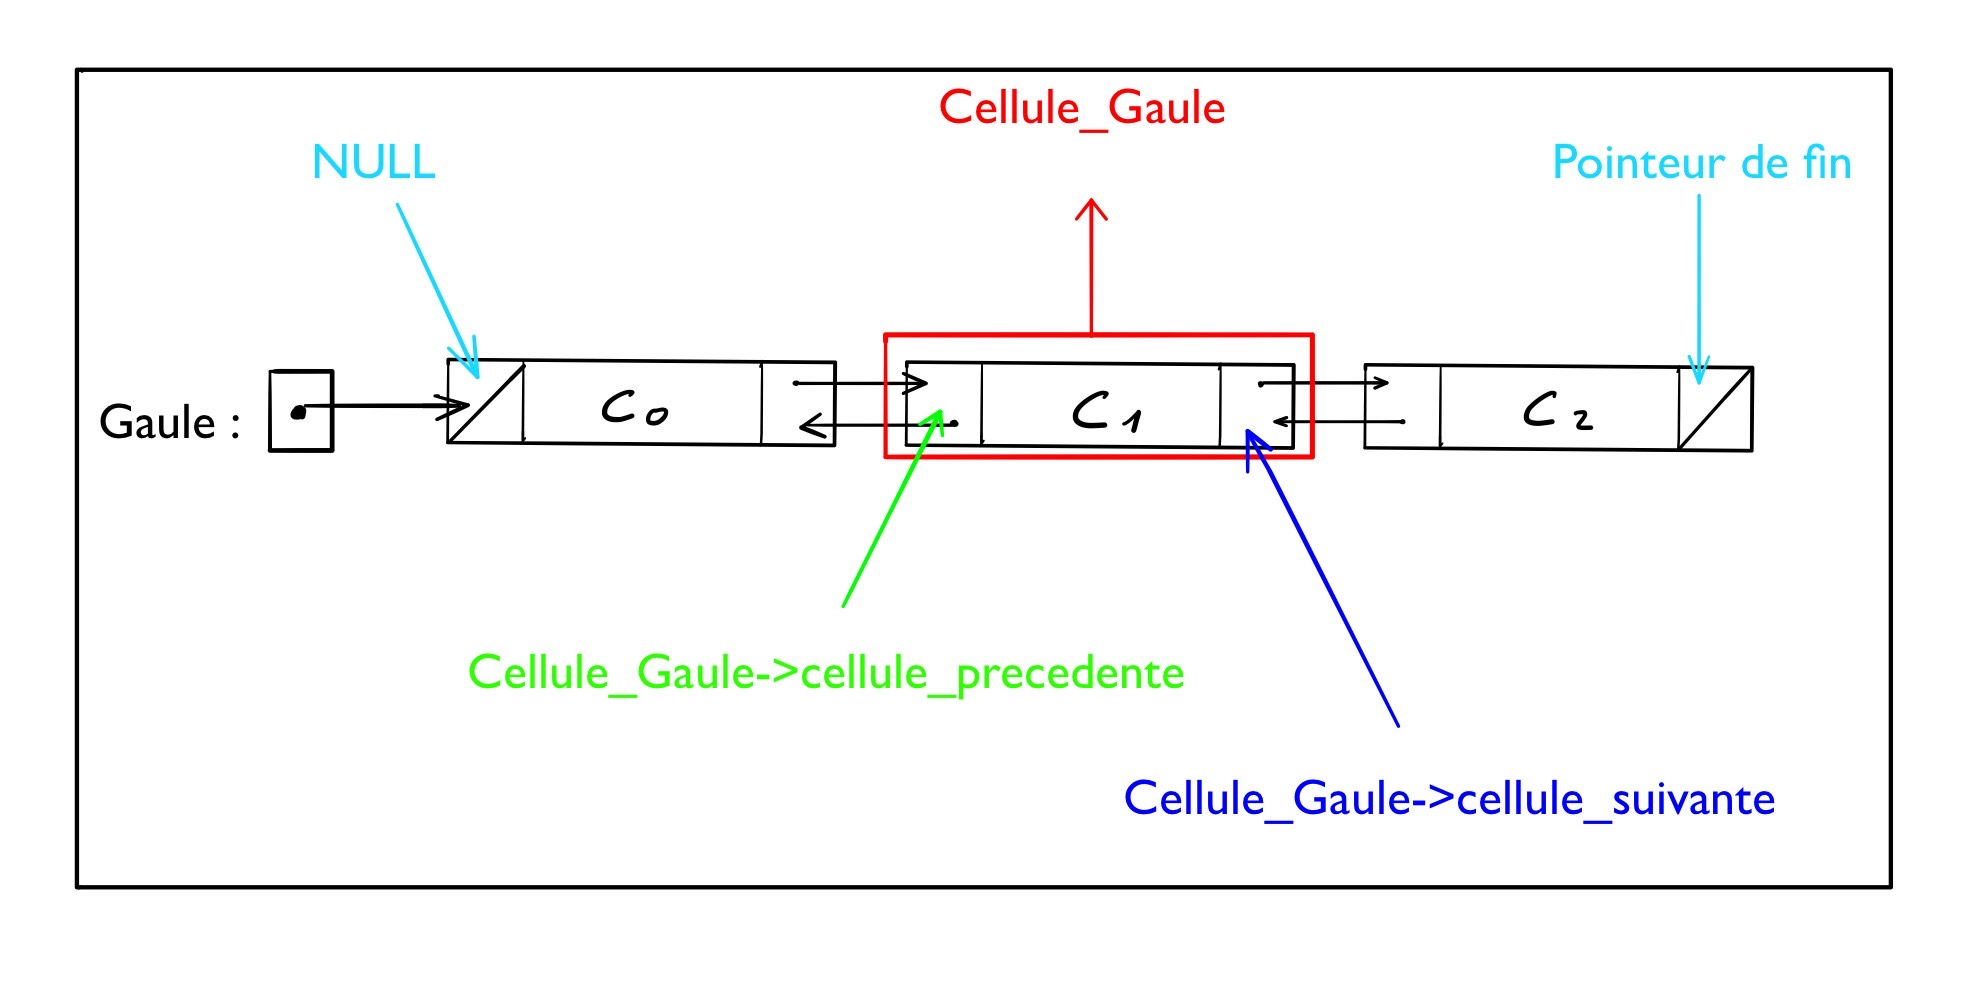
\includegraphics[scale=0.22]{schéma_liste_chainée.jpeg}
    \caption{Schéma de la strucutre sous forme de liste chainée}
\end{figure}

\section{\textbf{Implémentation des structures}}
\subsection{\textbf{Ville}}
Le header ville.h est implémenté par le ficher ville.c. Toutes les implémentations des fonctions/procédures 
sont très simples. En effet, la majorité d'entre elles ne sont que des accesseurs/setteurs et pour les autres 
il s'agit d'opérations mathématique ou d'allocation de mémoire très simple ayant toutes une complexité d'ordre O(1).
\subsection{\textbf{Gaule}}
\subsubsection{Tableau}
\begin{enumerate}
    \item accesseurs
    \\Comme pour ville, certaines fonctions sont uniquement des accesseurs/setteurs 
    et donc retourne une valeur d'un champ de Gaule. C'est notamment le cas des 
    fonctions/procédures : 
    \begin{itemize}
    \item \textbf{get\_nombre\_specialites} 
    \item \textbf{get\_est\_circuit} 
    \item \textbf{get\_nombre\_villes}
    \item \textbf{set\_nombre\_villes}
    \end{itemize}   
    \item Allocation de mémoire
    Une fonction et une procédure permettent l'allocation/libération de mémoire nécessaire à la 
    création/destruction des structures Gaule : 
    \begin{itemize}
        \item cree\_nouveau\_tour : alloue de la mémoire pour un nouveau tour. Cette fonction y crée 
        un pointeur vers un tableau pouvant contenir deux structures Ville, les deux villes étant données en argument y sont 
        intégrées si aucun échec d'allocation de mémoire n'a eu lieu. Le nombre de ville est initialisé à 2. 
        Par définition, le tour ne peut pas être une circuit lorsqu'il est nouvellement créé comme le spécifie l'énoncé. 
        Le champ est\_circuit est donc initialement nul.
        \item detruit\_tour : libère la mémoire allouée à une structure Gaule.
    \end{itemize}
    \item \textbf{ajoute\_ville}
    \\Cette fonction va s'occuper d'ajouter au tableau de villes, la ville donnée en argument 
    en s'assurant que celle-ci n'est pas la même que la dernière du tableau. Elle va également 
    s'occuper de mettre à jour certains champs de la structure Gaule(est\_circuit, nombre\_villes et 
    nombre\_specialites)
    \begin{itemize}
        \item SP1 : Vérification que l'on ne rajoute pas la même ville que la dernière de la liste.
        \item SP2 : Mise à jour du nombre de ville du tour
        \item SP3 : Aggrandissement de l'espace mémoire de tableau ville et ajout de la nouvelle ville
        \item SP4 : Mise à jour du nombre de spécialités et du champ de Gaule permettant de savoir 
        si le tour est un circuit ou non
    \end{itemize}
    \item \textbf{supprime\_ville}
    \\A l'inverse de ajoute\_ville, cette procédure retire la dernière ville du tableau à
    qu'il ne soit pas vide.
    \begin{itemize}
        \item SP1 : Mise à jour du nombre de spécialités et du nombre de villes
        \item SP2 : Realloue la mémoire du tableau afin d'en retirer la dernière ville
        \item SP3 : Mise à jour du champ de Gaule permettant de savoir si le tour est un circuit ou non
    \end{itemize}
    \item \textbf{compare\_string}
    \\Cette fonction permet de savoir si les 2 chaines de caractères données en argument 
    sont les mêmes. Pour ce faire, on compare tous caractères un à un de la première chaine 
    avec ceux respectifs de la deuxième.
    Ce problème va donc parcourir au Maximum l'entièreté de la première chaine de caractères.
    \\Voici le code étant solution de ce problème, agrémenté de son invariant de boucle.
    Spécifions pour ce problème $\forall s\in string, \exists i\in Entier, taille(s)=i, s[i-1]=0$
    \begin{lstlisting}[caption = {code comparaison de 2 chaines de caractères}]
    int i=0;
    (>\textcolor[HTML]{17983b}{\{$Inv: chaine1=chaine1_0\wedge chaine2=chaine2_0\wedge 0\leq i\leq length(chaine1)$\}}<)
    while(chaine1[i]!=0){
        (>\textcolor[HTML]{17983b}{\{$Inv\wedge B: chaine1=chaine1_0\wedge chaine2=chaine2_0\wedge 0\leq i<length(chaine1)$\}}<)
        if (chaine2[i]==0 || (chaine1[i]!=chaine2[i]))
            return -1;
        i++;
    }
    (>\textcolor[HTML]{17983b}{\{$Inv\wedge \lnot B \implies chaine1=chaine1_0\wedge chaine2=chaine2_0\wedge i=length(chaine1)$\}}<)
    if(chaine2[i-1]!=0)
        return -1;
    return 0;
    \end{lstlisting}
    \item \textbf{maj\_est\_circuit}
    \\Cette procédure redéfinit le booléen du champ est\_circuit de Gaule. Dans le cas où le tour contient
    au moins 3 villes, elle compare le nom de la première et dernière ville. Le tour est un circuit s'ils 
    correspondent.
    \item \textbf{get\_specialite}
    \\Cette fonction retourne la specialite de la ville dont le nom a été donné en argument. Pour se faire, 
    la fonction parcours le tableau de villes et compare leur nom un à un avec le nom donné. Si la 
    ville est trouvée dans le tour, on utilise l'accesseur créé à cet effet pour rendre la spécialité.
    \\Voici le code étant solution de ce problème, agrémenté de son invariant de boucle.
    \begin{lstlisting}[caption = {code boucle trouver ville correspondante}]
    int i = 0;
    (>\textcolor[HTML]{17983b}{\{$Inv: nom\_ville=nom\_ville_0\wedge 0\leq i\leq get\_nombre\_villes(tour)$\}}<)
    for(; i<get_nombre_villes(tour) && ville_appartient_tour==0; i++){
        (>\textcolor[HTML]{17983b}{\{$Inv\wedge B: nom\_ville=nom\_ville_0\wedge $}<)
        (>\textcolor[HTML]{17983b}{$0\leq i< get\_nombre\_villes(tour)\wedge ville\_appartient\_tour=0$\}}<)
        nom2 = get_nom_ville(tour->tableau_ville[i]);
        if(!compare_string(nom_ville, nom2)){
            ville_appartient_tour = 1;
            /*décrémente i de 1 car sera à nouveau incrémenter en fin de 
            boucle malgré que la boucle s'arrête dû à 
            ville_appartient_tour=1, ainsi i sera bien l'indice du tableau 
            où trouver la ville après la boucle*/
            i--;
        }
    }    
    (>\textcolor[HTML]{17983b}{\{$Inv\wedge \lnot B \implies nom\_ville=nom\_ville_0\wedge $}<)
    (>\textcolor[HTML]{17983b}{$(i=get\_nombre\_villes(tour)\vee (ville\_appartient\_tour=1\wedge 0\leq i< get\_nombre\_villes(tour)))$\}}<)
    \end{lstlisting}
    \item \textbf{ville\_en\_double}
    \\Cette fonction à pour objectif de définir si la ville donnée en argument apparait plus d'une fois 
    ou non dans le tour. On parcourt alors le tableau de villes afin d'y dénombrer le nombre d'occurance
    de la ville en question et enfin retourner un booléen correspondant.
    \\Voici le code étant solution de ce problème, agrémenté de son invariant de boucle.
    \begin{lstlisting}[caption = {code boucle nombre d'apparition d'une ville}]
    int n_apparition = 0;
    (>\textcolor[HTML]{17983b}{\{$Inv: nom\_ville=nom\_ville_0\wedge 0\leq i\leq get\_nombre\_villes(tour)\wedge $}<)
    (>\textcolor[HTML]{17983b}{$n\_apparition\leq 2\}$}<)
    for(int i = 0; i<get_nombre_villes(tour) && n_apparition<2 ; i++){
    (>\textcolor[HTML]{17983b}{\{$Inv\wedge B: nom\_ville=nom\_ville_0\wedge 0\leq i< get\_nombre\_villes(tour)\wedge $}<)
    (>\textcolor[HTML]{17983b}{$n\_apparition<2\}$}<)
    if(compare_string(get_nom_ville(tour->tableau_ville[i]),nom_ville)==0)
        n_apparition++;
    } 
    (>\textcolor[HTML]{17983b}{\{$Inv\wedge \lnot B\implies nom\_ville=nom\_ville_0\wedge (i=get\_nombre\_villes(tour)\vee $}<)
    (>\textcolor[HTML]{17983b}{$n\_apparition=2\}$}<)    
    \end{lstlisting}
\end{enumerate}

\subsubsection{Liste chainée}
\begin{enumerate}
    \item Accesseurs 
    \\De même que pour l'implémentation sous forme de tableau, certaines fonctions/procédures
    (précisées ci-dessous) ne requierent pas d'explications supplémentaires dû à leur simplicité. 
    Elles sont d'ailleurs également toutes de complexité O(1).
    \begin{itemize}
        \item \textbf{set\_nombre\_villes}
        \item \textbf{get\_nombre\_villes}
        \item \textbf{get\_est\_circuit}
        \item \textbf{get\_nombre\_specialites}
    \end{itemize}
    \item Allocation de mémoire
    \\Quatre fonctions, s'occupe de l'allocation de mémoire des structures Gaule et 
    \\Cellule\_Gaule. 
    \begin{itemize}
        \item \textbf{cree\_Cellule\_Gaule} : alloue de la mémoire pour une nouvelle cellule Cellule\_Gaule.
        Si l'opération n'a pas échouée alors elle y intègre également les informations données en argument.
        \item \textbf{detruit\_liste} : Cette fonction a pour but de libérer la mémoire des cellules 
        de la liste. Dû à son fonctionnnement récurssif, elle permet de libérer toutes les cellules depuis celle donnnée 
        en argument jusqu'à la dernière de la liste.
        \\En effet : $\forall C \in Cellule\_Gaule$
        \\detruit\_liste(C)=detruit\_liste(C$\rightarrow$cellule\_suivante)+free(C) 
        \\si C$\rightarrow$cellule\_suivante$\ne$NULL
        \\sinon detruit\_liste(C)=free(C)
        \item \textbf{cree\_nouveau\_tour} : alloue de la mémoire pour un nouveau tour. Cette fonction 
        fait également appel à cree\_Cellule\_Gaule avant d'intégrer les 2 premières villes du tour 
        données en argument à la liste nouvellement créer et donc permettre d'initialiser les champs 
        du nouveau tour lié à cette liste.
        \item \textbf{detruit\_tour} : Libère la mémoire allouer à un struct Gaule donnée en argument. 
        Elle y libère également la liste incluse à l'aide de la fonction créée à cet effet.
    \end{itemize}
    \item \textbf{ajoute\_ville}
    \\Cette fonction va ajouter une nouvelle cellule à la fin de la liste de cellule contenue dans le 
    tour et y mettre à jour certaines champ de tour.
    \begin{itemize}
        \item SP1 : Vérification que l’on ne rajoute pas la même ville que la dernière de la liste.
        \item SP2 : Incrémentation de 1 le champ contenant le nombre de villes du tour
        \item SP3 : Création d'une nouvelle cellule contenant la nouvelle ville
        \item SP4 : pointeur de cellule suivante de la cellule précédant la nouvelle cellule et pointeur 
        de dernière cellule du tour mis à jour
        \item SP5 : Mise à jour du nombre de spécialités et du champ de Gaule permettant de savoir
        si le tour est un circuit ou non
    \end{itemize}
    \item \textbf{supprime\_ville}
    \\La dernière cellule de la liste chainée est retirée et libérée à l'aide de cette procédure. Elle met 
    également à jour les champs du tour nécessitant un changement.
    \begin{itemize}
        \item SP1 : Mise à jour du nombre de spécialités et du nombre de villes
        \item SP2 : Libère la dernière cellule et met à jour le pointeur de dernière cellule du tour
        sur la cellule précédant l'ancienne dernière.
        \item SP3 : Mise à jour du champ de Gaule permettant de savoir si le tour est un circuit ou
        non
    \end{itemize}
    \item \textbf{maj\_est\_circuit}
    \\Cette procédure vérifie, dans le cas où le tour est constitué d'au moins 3 villes, la correspondance 
    des noms de la première et dernière ville afin de revoyer un booléen correspondant à cette vérification.
    \item \textbf{get\_specialite}
    \\Cette fonction renvoit la spécialité de la ville dont le nom est donné en argument.
    \begin{itemize}
        \item SP1 : Chercher la ville parmis la liste contenue dans le tour
        \item SP2 : Renvoyer le nom de la specialite de la ville si elle est trouvée
    \end{itemize}
    SP1$\implies$SP2
    Le SP1 implique l'utilisation d'une boucle où l'on compare le nom de la ville de la cellule 
    actuelle avec le nom donné. Tant qu'ils ne correspondent pas, notre cellule devient la cellule 
    suivante. Notre invariant se traduirait alors comme ceci
    \\$Inv : 1\leq i \leq get\_nombre\_villes(tour)+1$ avec i correspondant à la ième cellule de la liste.
    \item \textbf{ville\_en\_double}
    \\Cette fonction à pour objectif de définir si la ville donnée en argument apparait plus d’une
    fois ou non dans le tour. On parcourt alors le tableau de villes afin d’y dénombrer le nombre
    d’occurance de la ville en question et enfin retourner un booléen correspondant.
    Pour se faire, on parcourt la liste par chaque cellule en partant de la première jusqu'à la fin ou jusqu'à
    avoir au moins trouver deux cellules dont le nom de la ville correspond au nom donné en argument.
    Elle renvoit alors le booléen correspondant au fait que la ville s'y trouve au moins deux fois ou non.
    \item \textbf{compare\_string}
    Cette fonction correspond parfaitement à la fonction de l'implémentation sous forme de tableau. Son 
    implémentation est donc détaillée dans la section 4.2.1 point 4 et également dans l'Extrait 
    de Code 6 s'y trouvant.
\end{enumerate}

\section{\textbf{Complexité}}

\section{\textbf{Avantage et Inconvénients entre liste et tableau}}
Nous pouvons constater des différences notables entre les deux implémentations.

\paragraph{} Premièrement, il est nettement plus facile d'accéder à un élément du tableau, qui se fait 
de manière directe, comparé à la liste qui nécessite dans tous les cas de parcourir toutes la liste 
jusqu'à l'élément recherché.

\paragraph{} Par ailleurs, la liste a pour net avantage la gestion de ses cellules qui permet l'ajout et le retrait 
d'une ville très facilement comparé au tableau qui, pour se faire, devra impliquer une réallocation de mémoire, 
telle est la technique que j'ai décidé d'adopter, ou la recréation complete d'un nouveau tableau aux nouvelles dimensions. 
Dans mon implémentation, j'ai fixé comme règle que l'ajout ou le retrait ne se fait uniquement à la dernière position 
dans les deux cas, ce qui rend la liste d'autant plus pratique dès lors que je garde en mémoire l'adresse de sa 
dernière cellule. Si j'avais accordé à l'utilisateur de donner l'indice de l'endroit ou ajouter/retirer un cellule, 
alors il serait paru comme inconvénients pour la liste de devoir parcourir cette dernière jusqu'à la cellule se trouvant à cet indice.

\paragraph{} Enfin, notons une très légère augmentation de l'espace mémoire nécessaire à une liste dont chacunes 
de ses cellules contient deux pointeurs supplémentaires. Cette différence ne serait qu'un véritable inconvénients qu'en cas 
de liste d'une taille très importante.

\end{document}